\documentclass[]{report}
\usepackage[utf8]{inputenc}
\usepackage{graphicx}
\graphicspath{{graphics/}}


% Title Page
\title{
	SwingGame\endgraf
	Third Year Project Report
}
\author{
	\parbox{\linewidth}{
		\centering%
		Tim Brier\endgraf
		School of Computer Science\endgraf
		University of Manchester
	}
}
% Abuse the date to add extra info to the title page
\date{
	\parbox{\linewidth}{
		\centering%
		April 2015\endgraf\bigskip
		Supervised by Dr Steve Pettifer
	}
}


\begin{document}

\maketitle

\begin{abstract}
This paper details the development of SwingGame, a 2D video game in which players use ropes and grappling hooks to get to a goal in various levels.  The SwingGame project had two main goals, to produce a reusable framework for building games and to produce a fun and engaging game using that framework. The goals were successfully achieved with the framework being used for multiple finished products and SwingGame receiving praise by those who have seen and played it.
\end{abstract}

\tableofcontents


\chapter{Context}
This chapter provides an overview of what the project contains and its main goals. Similar existing technology is discussed along with why the decision to make a new system was made.
	\section{Project Description}
	The main system produced in this project is the game framework. This framework should handle all tasks generic to every video game including window management, drawing to the window and event handling. The framework should be easy to use, a developer should be able to define just the level and player behaviour and have a working game. It should also be extensible so that if any future projects require more complex features they can be easily added in.
	
	SwingGame was built using and alongside this framework. The game consists of a number of levels, each containing several obstacles and a goal. The aim of each level is to travel from the players starting point to the goal of the level using the physics of swinging around the various obstacles. Levels are scored based on the time it took for the player to reach the goal. The main objective of SwingGame is to show that the game framework is usable, but ideally it should also be an entertaining and engaging game.
	\section{Existing Technologies}
	This section discusses existing technology similar to this project. The technologies include other game frameworks and existing games which incorporate similar swinging mechanics.
		\subsection{Game Frameworks}
		There already exists several game frameworks (sometimes called engines) which have a variety of different feature sets. The most popular and most similar of these frameworks are discussed here.
			\subsubsection{Popular Frameworks}
			The most popular publicly available frameworks in use today are Unity\cite{unity} and Unreal Engine\cite{unreal}. Both of these frameworks are extremely powerful and complex. They focus more on 3D environments, providing systems to create game worlds and accurate real world physics simulation. These engines have historically been used in large projects with teams of developers but are now starting to be adopted by single developers due to more relaxed licensing fees.
			\subsubsection{Similar Frameworks}
			GameMaker\cite{gamemaker} is a framework more similar to the one in this project in that it is used for 2D games but it is also a lot more complex. It provides an entire language for developers to use to create games and includes GUI systems which allow developers to make games with minimal coding.
			
			A much more similar framework to the one in this project is Löve\cite{love}. Löve allows developers to script the behaviour of 2D games in Lua and provides modules to handle common game tasks including drawing, event handling and physics.
			\subsubsection{Decision To Make A New Framework}
			Most of the frameworks discussed previously were too complex for the needs of SwingGame. This project did not need a whole suite of tools for creating worlds and animations so the most likely candidate to use was Löve. However the decision was made to create a new framework for the project, mostly as a learning exercise. The Dragonfly project shows that "game engines present the opportunity to strengthen programming skills and expose students to a range of fundamental computer science topics"\cite{dragonfly}. Also, the most interesting component of this project, implementation wise, was the physics of the game. If an existing physics system was used the SwingGame project would have been too simple.
			
		\subsection{Games}
		Several games exist which have similar swinging mechanics to SwingGame. This section will discuss how some of those games use swinging and how they differ from SwingGame.
			\subsubsection{Spider-Man}
			Various Spider-Man games have used swinging on a line web to get around the environment, one of which is Spider-Man 2\cite{spiderman} by Treyarch. In this game the player uses the swinging mechanic to quickly navigate around a 3D virtual New York City.
			\subsubsection{Worms}
			The Worms\cite{worms} series by Team17 includes an item called the Ninja Rope. This item is used to attach to scenery in the level and swing the character to areas that would have otherwise been inaccessible. The swinging in these games was the biggest inspiration for SwingGame so it behaves very similarly to the swinging in SwingGame.
			\subsubsection{Floating Point}
			Floating Point\cite{floatingpoint} is a game by independent developer Tom Francis. This game is built upon using swinging to move around a 2D level, much like SwingGame. The player must use swinging to gain speed which makes several bars in the level grow taller. When the player crosses paths with one of these bars they collect points, the taller the bar the more points it scores.
			\subsubsection{Differences With SwingGame}
			While the swinging movement in SwingGame is very similar to that of the Worms games and Floating Point it differs in objective to all of the discussed games. The other games all use swinging to move generally through the level and don't enforce a specific goal area. In SwingGame the entire aim of each level is to navigate around the various obstacles to reach one specific goal point in the level, making each level into a puzzle for the player to solve.

\chapter{Design}
	\section{Requirements}
		\subsection{Features}
	\section{Technologies Used}
		\subsection{Language}
		\subsection{Libraries}
	\section{Game Design}


\chapter{Development}
This chapter outlines the development process of the project. It discusses some decisions which were made during implementation and the modules created. Some implementation detail is provided for the more interesting parts of the project.

	\section{SFML Abstractions}
	When implementation of the project began it was decided that there should be a layer of abstraction between the game framework and SFML. This decision was made initially because it was always possible that the classes provided by SFML would be missing some desired functionality. By putting a layer in between the framework and SFML any extra features could be implemented in this layer. This proved to be useful for adding a pause feature to the provided clock class among other enhancements.
	
	The way this abstraction was implemented was to create a class for each SFML class the framework used. The created class inherited from the SFML class and all uses of the class in the framework would use the new subclass. This meant than whenever functionality was added to an SFML subclass this functionality could be used by any existing instance of the class in the project without having to change its type.
	
	\section{Modules}
	This section details the various modules present in both the game framework and in SwingGame. A high level view of how each module works is provided as well as why each module is a part of either the game or the framework.
		\subsection{Game Framework}
		The modules contained in the game framework are those which are not dependant on the type of game being made. Whatever the end product is these tasks will always be performed in the same way.
			\subsubsection{Window Management}
			\subsubsection{Graphics}
			The requirements for graphics in this project were fairly straightforward, draw shapes and text to the screen. The most advanced graphics feature was being able to load an image into an object called a sprite which can move around the screen. This was mostly handled by SFML but some extra features were implemented. An image cache was created meaning that multiple sprites could share the same loaded image instead of duplicating it in memory. The ability to draw debug features of shape was also implemented. The graphics module could draw the origin of each shape along with all the points that make up that shape. A very useful piece of debug information which could be drawn was the bounding box of a shape, the smallest axis aligned rectangle which contains the entire shape. This bounding box is used in collisions and being able to see it proved very useful when working on collisions.
			\begin{figure}[h]
				\centering
				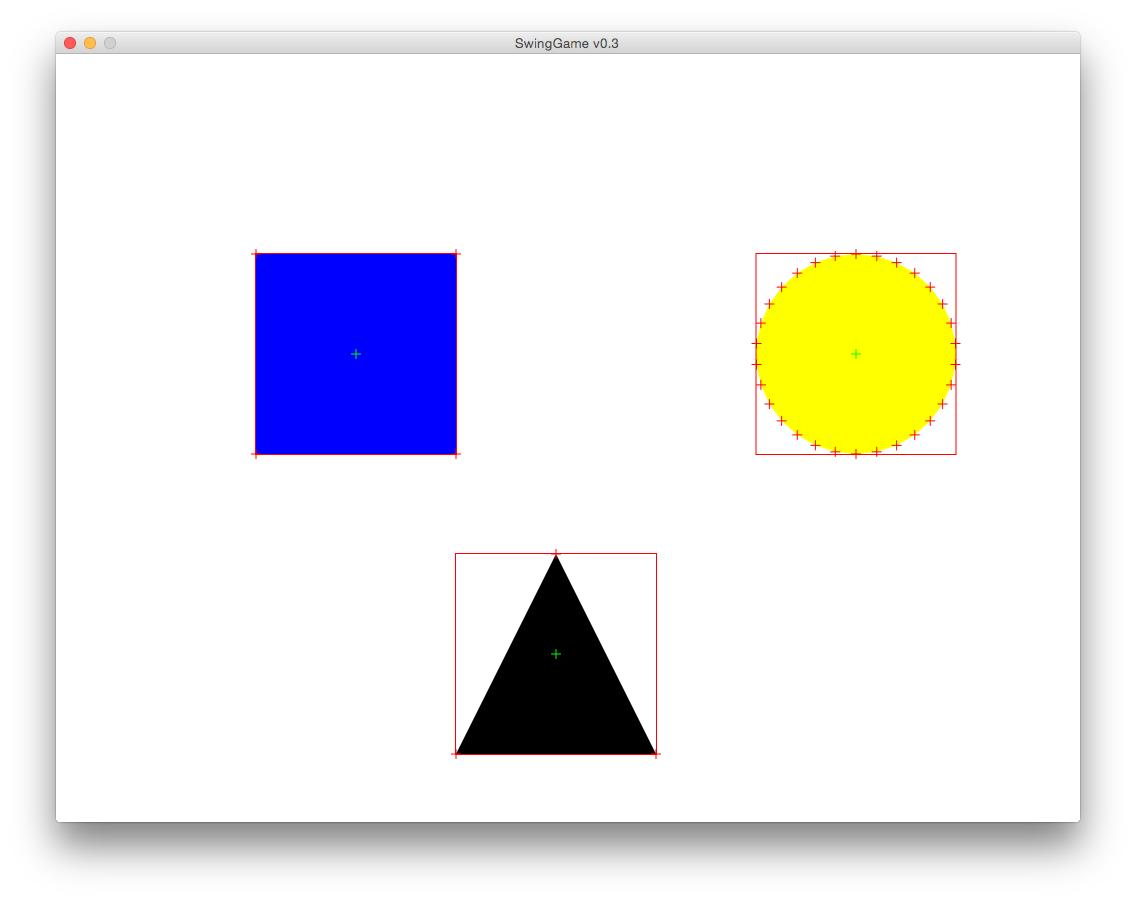
\includegraphics[scale=0.25]{debuggraphics}
				\caption{A simple scene with debug graphics being drawn}
				\label{debuggraphics}
			\end{figure}
			
			\subsubsection{Gameloop}
			\subsubsection{Event Management}
			\subsubsection{Menu System}
			\subsubsection{Collision Detection}
		\subsection{SwingGame}
	

\chapter{Evaluation}
	\section{External Testing}
	\section{Use In Other Projects}
	

\chapter{Reflection and Conclusion}
	\section{Achievements}
	\section{Lessons Learned}
	\section{Future Improvements}
	
\bibliographystyle{plain}

\bibliography{sources}

\end{document}          
